%%%%%%%%%%%%%%%%%%%%%%%%%%%%%%%%%%%%%%%%%%%%%%%%%%%%%%%%%%%%%%%%%%%%%%%%%%%%%
%
% This is a LaTeX file for an A0 poster.
%
% template poster taken from https://canizo.org/latex_poster
%
%%%%%%%%%%%%%%%%%%%%%%%%%%%%%%%%%%%%%%%%%%%%%%%%%%%%%%%%%%%%%%%%%%%%%%%%%%%%%

%%%%%%%%%%%%%%%%%%%%%%%%%%%%%%%%%%%%%%%%%%%%%%%%%%%%%%%%%%%%%%%%%%%%%%%%%%%%%
%%%%%%%%%%%%%%%%%%%%%%%%%%%%%%%%%%%%%%%%%%%%%%%%%%%%%%%%%%%%%%%%%%%%%%%%%%%%%
%
% msdata2 poster for the Eurobioc2019, December 2019.
%
%%%%%%%%%%%%%%%%%%%%%%%%%%%%%%%%%%%%%%%%%%%%%%%%%%%%%%%%%%%%%%%%%%%%%%%%%%%%%
%%%%%%%%%%%%%%%%%%%%%%%%%%%%%%%%%%%%%%%%%%%%%%%%%%%%%%%%%%%%%%%%%%%%%%%%%%%%%

\documentclass{article}
% To modify the size of the page:
\usepackage[dvips,a3paper,portrait,centering,margin=0.4cm]{geometry}
% To create multiple columns
\usepackage{multicol}

\usepackage[utf8]{inputenc}
% To align images
\usepackage[export]{adjustbox}
% Use captions in minipages
\usepackage{caption}
% Math font
\usepackage{amsmath, amsthm, amsfonts}
% Include figure files.
\usepackage{graphicx}

\usepackage{hyperref}
\usepackage{breakurl}
\hypersetup{%
  pdfauthor={Chong Tang and Laurent Gatto},%
  pdfusetitle,
  bookmarks = {true},
  bookmarksnumbered = {true},
  bookmarksopen = {true},
  bookmarksopenlevel = 2,
  unicode = {true},
  breaklinks = {false},
  hyperindex = {true},
  colorlinks = {true},
  linktocpage = {true},
  plainpages = {false},
  linkcolor = {Blue},
  citecolor = {Blue},
  urlcolor = {Red},
  pdfstartview = {Fit},
  pdfpagemode = {UseOutlines},
  pdfview = {XYZ null null null}
}


% Coding fonts
% ------------
% For including R chunks
\usepackage{listings}
\lstset{
  language=R,
  basicstyle=\small\ttfamily\color{vdgray},       % the size of the fonts that are used for the code
  % sensitive=false,
  numbers=left,                   % where to put the line-numbers
  numberstyle=\tiny\color{gray},  % the style that is used for the line-numbers
  stepnumber=1,                   % the step between two line-numbers.
  numbersep=0.1cm,                % how far the line-numbers are from the code
  backgroundcolor=\color{lgray},  % choose the background color. You must add \usepackage{color}
  deletekeywords={stat},
  keywordstyle=\color{blue},      % keyword style
  stringstyle=\color{green},      % string literal style
  xleftmargin=0.5cm,
}
% Create command for highlighting inline code or variables
\newcommand{\hcode}[2][lgray]{{\ttfamily\color{vdgray}\colorbox{#1}{#2}}}

% Colors
% ------
\usepackage{color}
\usepackage[dvipsnames]{xcolor}
% Color panel used throughout the poster
\definecolor{lgray}{rgb}{0.9179688,0.9179688,0.9179688} % #ebebeb
\definecolor{dgray}{rgb}{0.796875,0.796875,0.796875} % #cccccc
\definecolor{vdgray}{rgb}{0.3984375,0.3984375,0.3984375} % #666666
\definecolor{coral}{rgb}{0.9960938,0.4960938,0.3125000} % #ff7f50
\definecolor{blue}{rgb}{0.4218750,0.6484375,0.8007812} % #6ca6cd
\definecolor{green}{rgb}{0.6992188,0.7265625,0.5078125} % #b3ba82
\definecolor{yellow}{rgb}{0.9570312,0.8671875,0.6992188} % #f5deb3

% Adjust space between reference items
% ------------------------------------
\let\OLDthebibliography\thebibliography
\renewcommand\thebibliography[1]{
  \OLDthebibliography{#1}
  \setlength{\parskip}{0pt}
  \setlength{\itemsep}{0pt plus 0.3ex}
}

\pagestyle{empty}

\def\to{\rightarrow}


% ===========================================================================

\title{}
\author{}
\date{}

\begin{document}


% ---------------------------------------------------------------------------
% Banner


\begin{center}
  \colorbox{lgray}{
    \begin{minipage}[c]{3cm}
      
\includegraphics[width=12em]{pix/ucllogo.png}
    \end{minipage}%

  \begin{minipage}{.74\textwidth}
    \begin{center}
      % Title
      \huge \textbf{The \texttt{msdata2} data package for proteomics benchmarking} \\
      \vspace{0.4cm}
      % Authors
      \Large \textbf{Chong Tang, Laurent Gatto} \\
      % Affiliation
      \Large \textit{Computational biology and bioinformatics lab, de Duve Institute, UCLouvain } \\
      % email
      \vspace{0.4cm}
      \normalsize chong.tang@uclouvain.be -- laurent.gatto@uclouvain.be \\
    \end{center}
  \end{minipage}
  %&
  \begin{minipage}{5cm}
    
\includegraphics[width=9em]{pix/Institut_de_Duve.png}
  \end{minipage}
}
\end{center}


% ------------------------\---------------------------------------------------
% Summary

\setlength{\columnsep}{1cm}

\begin{multicols}{2}

\noindent
\fcolorbox{yellow}{yellow}{
  \begin{minipage}[t]{\linewidth}
      \vspace{.15cm}
      \section*{\huge Summary}

      \large The \hcode{msdata2} package contains a set of published
      quantification/identification proteomics datasets. The purpose
      of the package is to provide standard and curated datasets to
      facilitate the benchmarking of proteomics workflows.

  \end{minipage}
}


\noindent
\begin{minipage}[t]{\linewidth}
  \vspace{0.55cm}
  \section*{The SGS Datasets}
  \large

  The first dataset in \hcode{msdata2} is a SWATH experiment processed
  with OpenSWATH output from SGS dataset. The SWATH-MS Gold Standard
  (SGS) dataset consists of 90 SWATH-MS runs of 422 synthetic stable
  isotope-labeled standard (SIS) peptides in ten different dilution
  steps (1, 2, 4, 8, ..., 512 times), spiked into three protein backgrounds
  of varying complexity (water, yeast and human), acquired in three
  technical replicates \cite{Rost2014vh}.

  \vspace{1cm}

  \begin{center}
    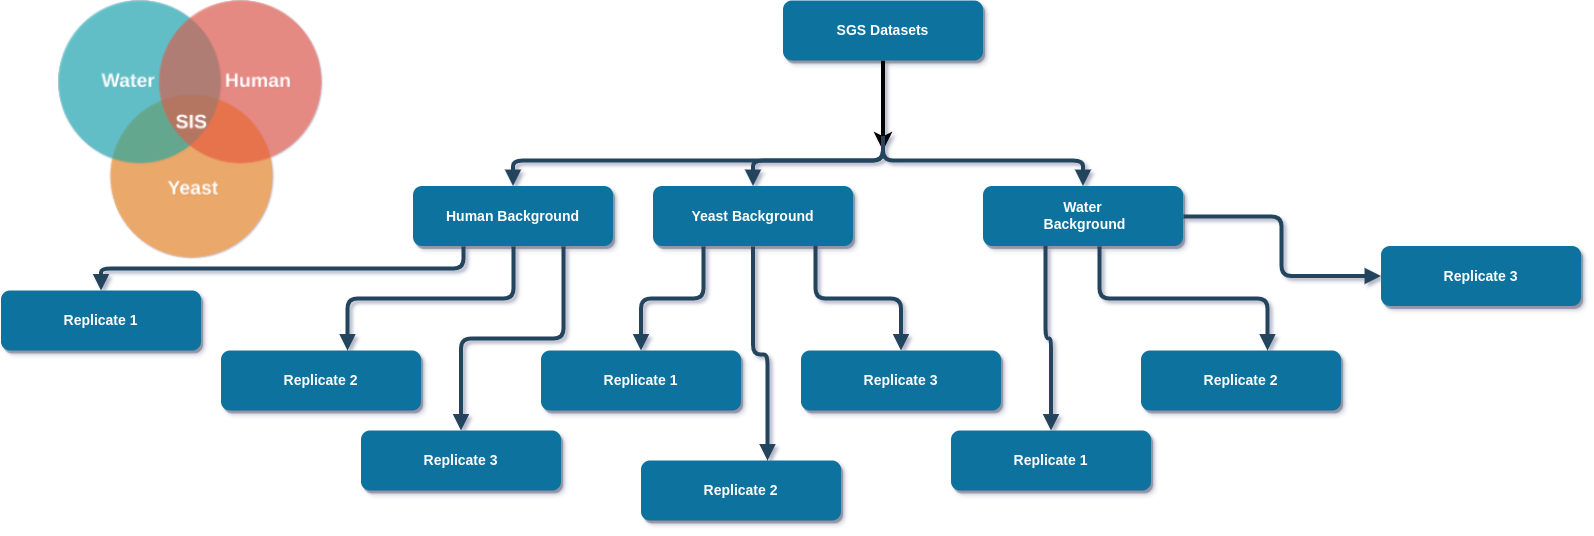
\includegraphics[width=\textwidth]{pix/DS.png}
  \end{center}

  \vspace{1cm}

  The SGS dataset was manually annotated, resulting in 342 identified
  and quantified peptides with three or four transitions each. In
  total, 30,780 chromatograms were inspected and 18,785 were annotated
  with one true peak group, whereas in 11,995 cases no peak was
  detected. The data were processed and converted into \hcode{MSnSet}
  objects \cite{MSnbase} (see below and on the right):

  \vspace{1cm}

  \begin{tabular}{@{\extracolsep{5pt}} ll}
    \\[-1.8ex]\hline
    \hline \\[-1.8ex]
    \textbf{Slot} & \textbf{Information} \\
    \hline \\[-1.8ex]
    assayData   & quantitative matrix with XIC values \\
    phenoData   & sample metadata \\
    featureData & feature metadata (identification data, peptides sequences, ...) \\
    experimentData & experimental methods and general annotations \\
    processingData & processing information and log \\
    \hline \\[-1.8ex]
  \end{tabular}

\end{minipage}




% \noindent
% \begin{minipage}[t]{\linewidth}
%   \vspace{0.5cm}
%   \large
%   \begin{center}
%     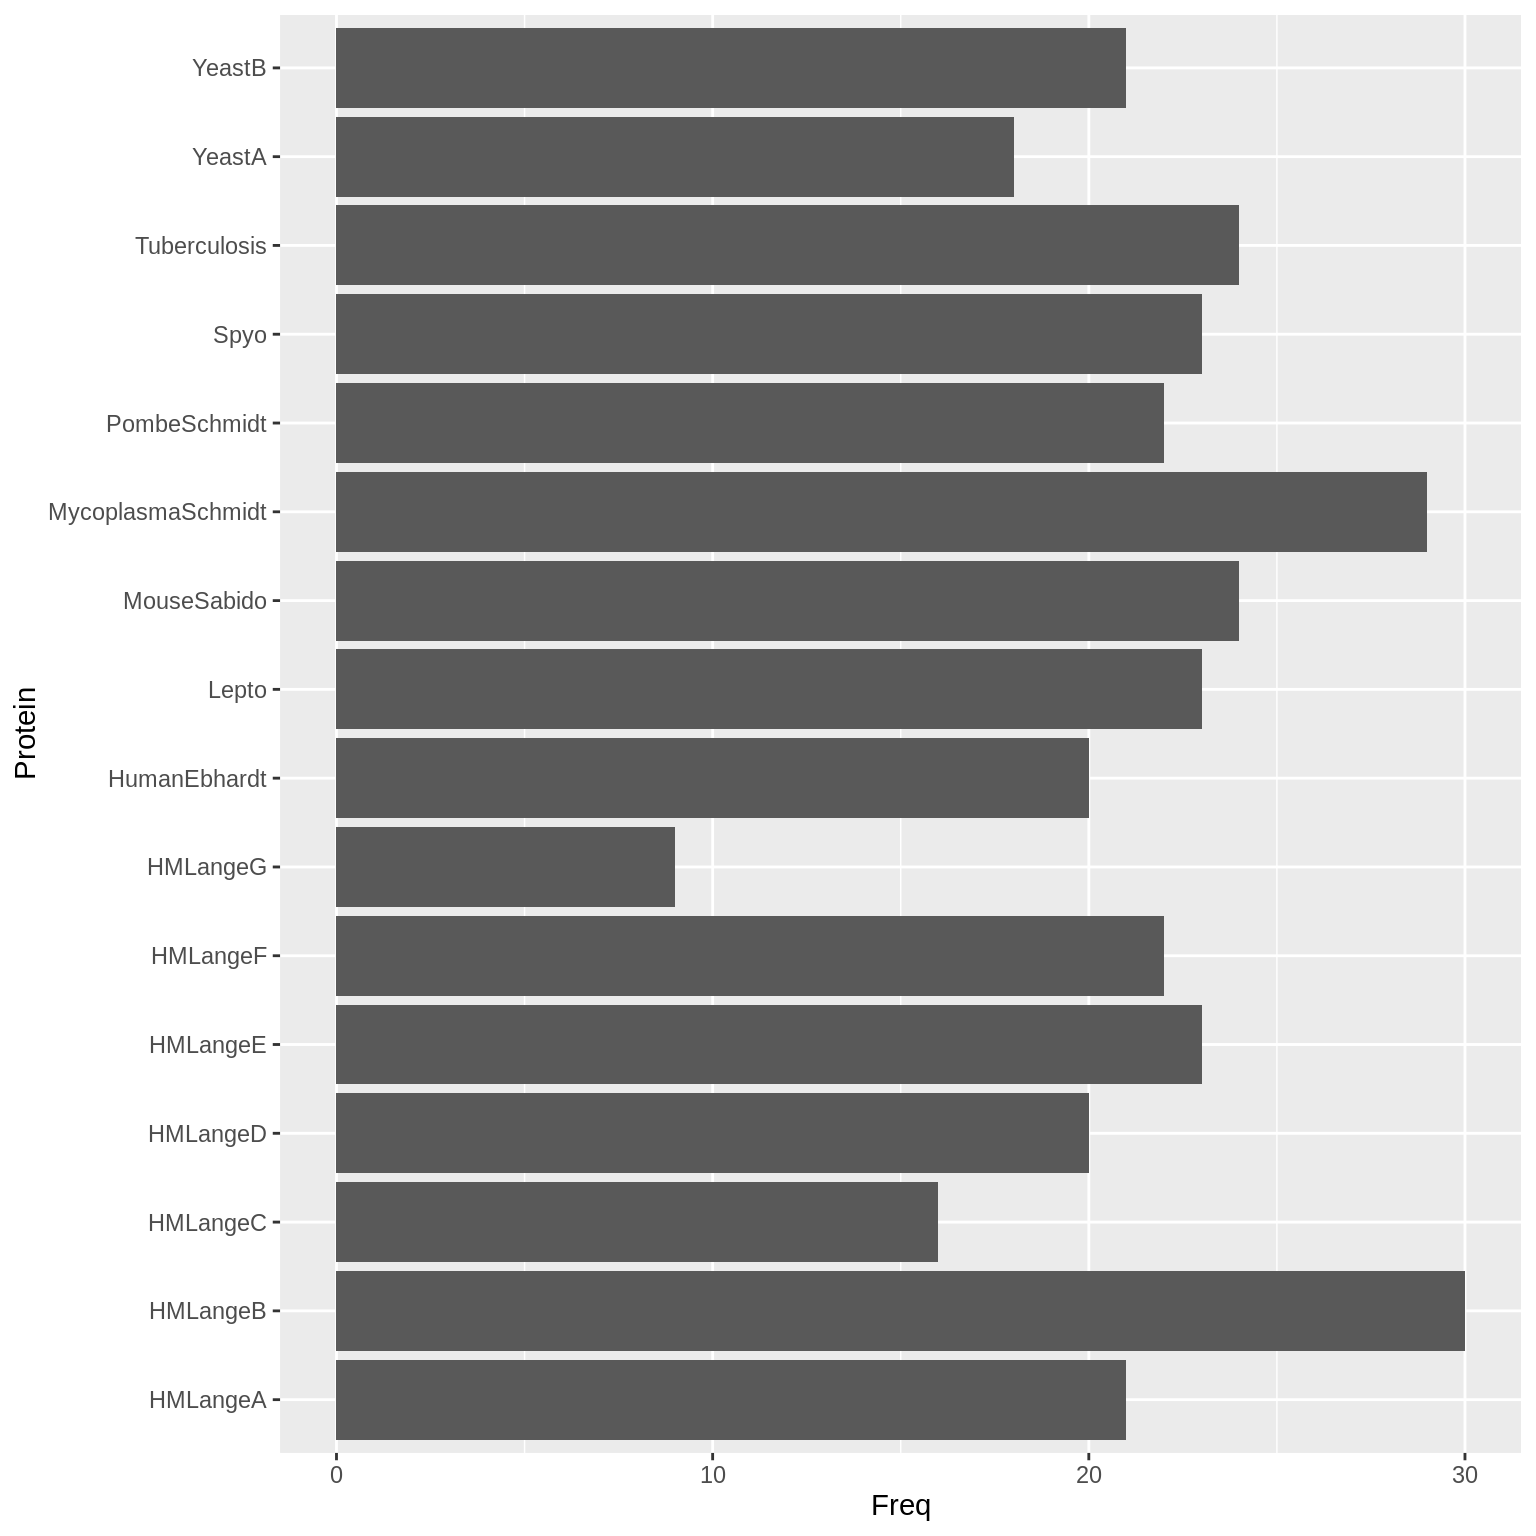
\includegraphics[width=0.6\textwidth]{pix/human3.png}
%   \end{center}
%   \vspace{-0.5cm}
%   \captionof{figure}{\textbf{Unique peptide count} for each protein in the human background.}
% \end{minipage}

\noindent
\begin{minipage}[h]{1\linewidth}
  \vspace{1cm}

  \section*{Handling raw MS data}
  \large

  The raw MS data in \hcode{msdata2} will be handled by \hcode{Spectra} package.
  The new \hcode{Spectra} package provides a common, flexible and a high-performance infrastructure to represent and handle MS data in R \cite{Spectra}. 
  Various open-formats, e.g. mzML, mzXML, mz5 from different vendors can all be supported by \hcode{Spectra}.
  The spectrum data (m/z - intensity pairs) will be represented as a matrix stored/provided by the Backend class.
  
  \vspace{1cm}

  \begin{tabular}{@{\extracolsep{0.5pt}} llll}
    \\[-1.8ex]\hline
    \hline \\[-1.8ex]
    \textbf{class} & \textbf{source.files} 
    & \textbf{storage} & \textbf{writeable}\\
    \hline \\[-1.8ex]
    MsBackendDataFrame & manual & in-memory & yes \\
    MsBackendHdf5Peaks & hdf5 & on-disk & yes \\
    MsBackendMzR & mzML, mzXML and CDF & on-disk & no \\
    MsBackendHmdbXml & XML & on-disk & yes \\
    MsBackendRawFileReader & Thermo .raw & on-disk & no \\
    \hline \\[-1.8ex]
  \end{tabular}
  

\end{minipage}



\vspace{.4cm}
\noindent
\colorbox{yellow}{
  \begin{minipage}[t]{0.965\linewidth}
    \vspace{.15cm}
    \section*{\huge Conclusion and Future Work}
    \large Our package \hcode{msdata2} will provide formatted labelled
    and label-free quantification and raw data for proteomics.  In the
    future, we will also include large raw MS data, making use of the
    ExperimentHub cloud infrastructure. Our goal is for
    \hcode{msdata2} to become a benchmarking tools on different
    computational proteomics workflows.

  \end{minipage}
}


\noindent
\begin{minipage}[h]{1\linewidth}
  \vspace{1cm}

  \section*{Data exploration}
  \large

  Data visualization on the \hcode{MSnSet} with Human background. We
  can notice the good consistency between replicates. The principal
  component analysis confirms good separation for runs 10 to 7 (up to
  dilution 8x). Further dilutions become much more difficult to tell
  apart.

\end{minipage}

\begin{minipage}[h]{\linewidth}
\hspace{0.4cm}
  \begin{center}
    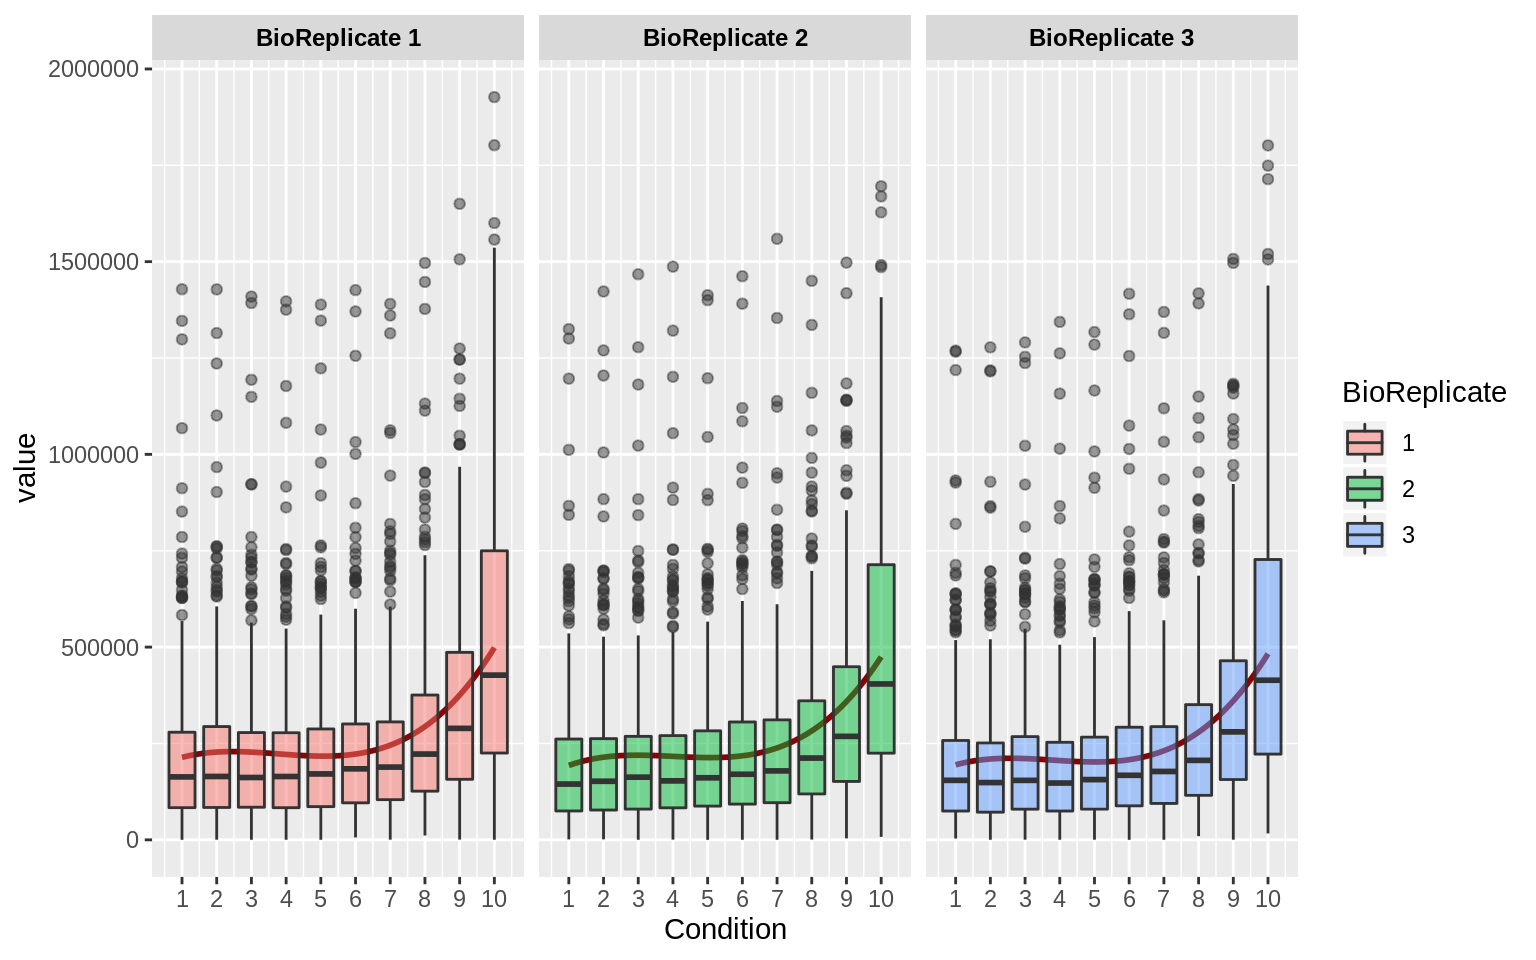
\includegraphics[width=0.45\linewidth]{pix/human1.png}
    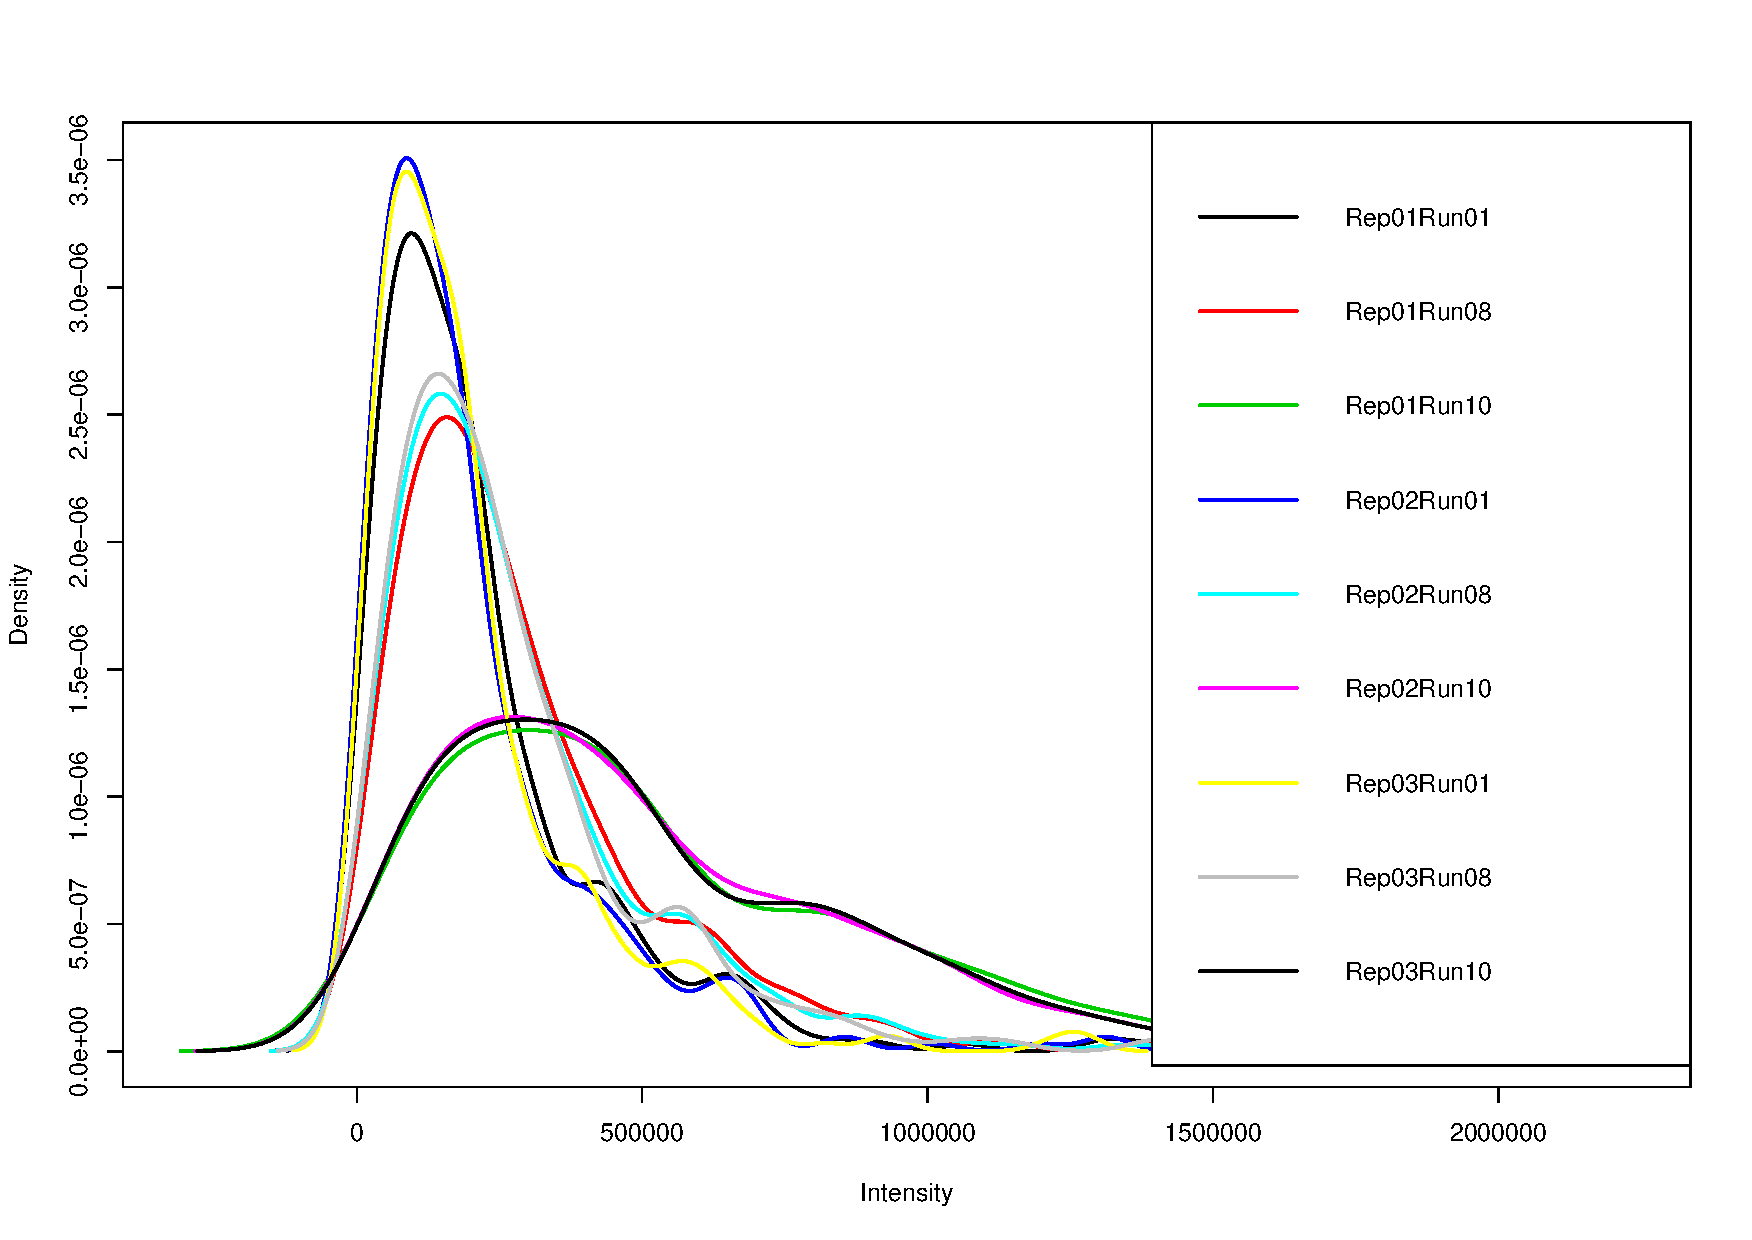
\includegraphics[width=0.45\linewidth]{pix/human2.pdf}
    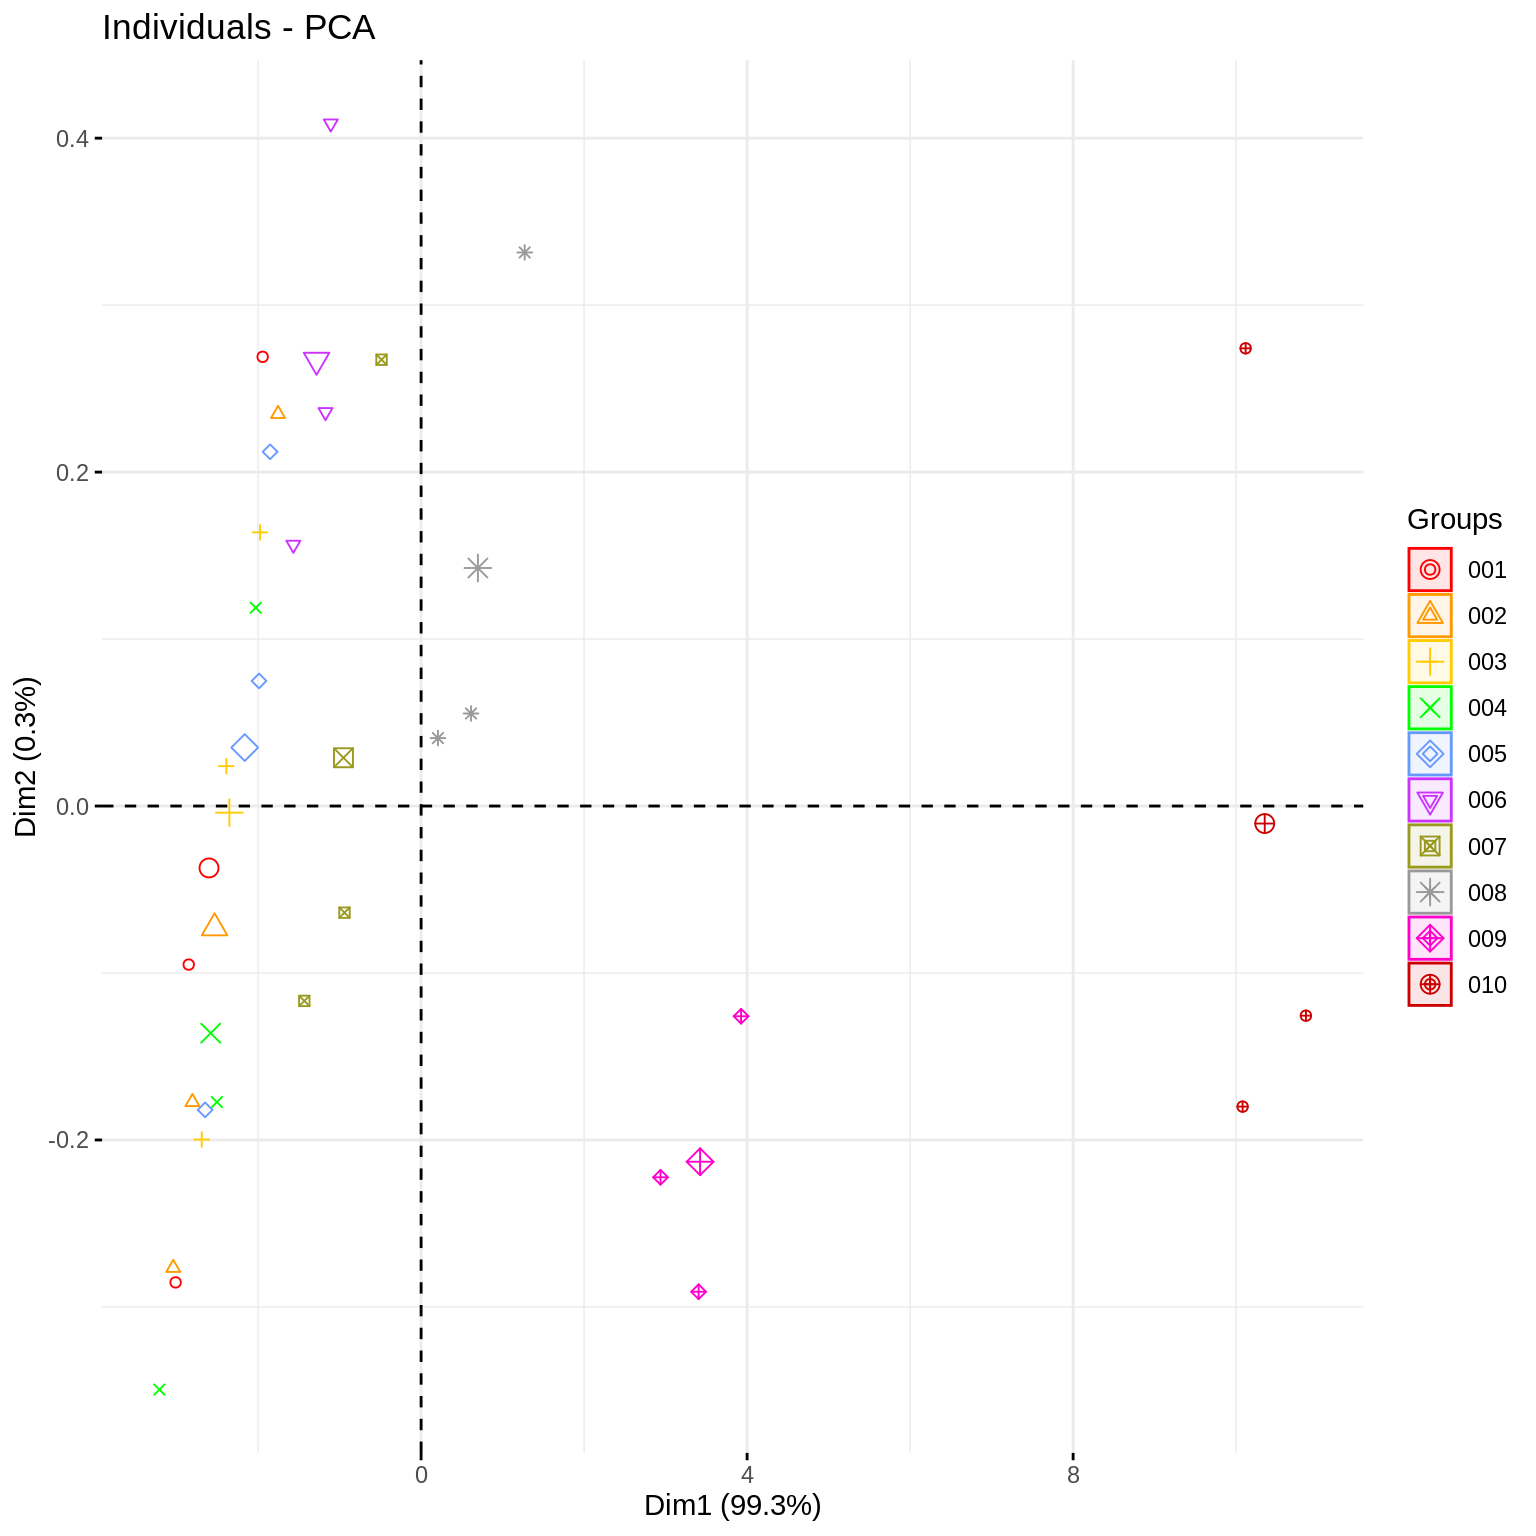
\includegraphics[width=0.4\linewidth]{pix/PCA.png}
    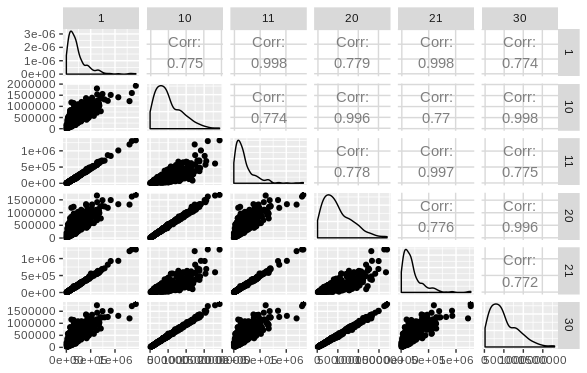
\includegraphics[width=0.5\linewidth]{pix/ggpairs.png}
  \end{center}

\end{minipage}
\noindent

\noindent
\begin{minipage}[t]{\linewidth}
  \vspace{0.55cm}
  \section*{Data preparation}
  \large

  \begin{center}
    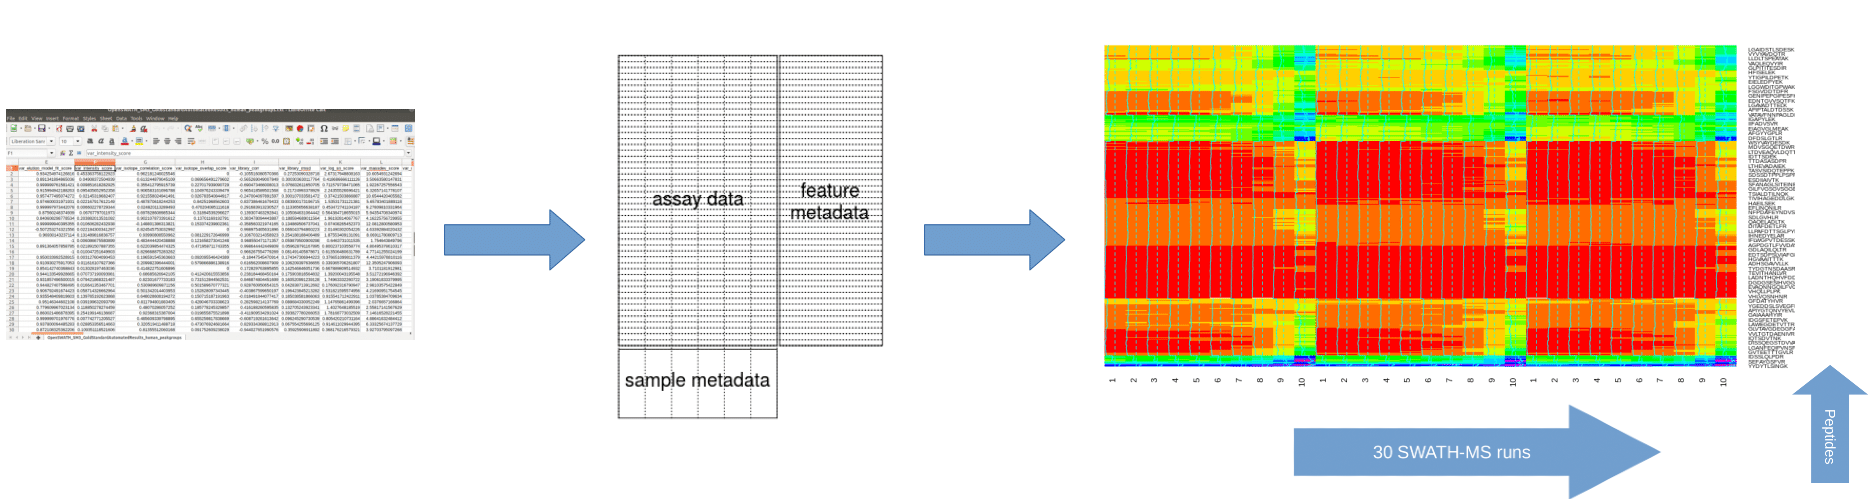
\includegraphics[width=0.95\textwidth]{pix/WF1.png}
  \end{center}
  \vspace{-0.5cm} \captionof{figure}{The OpenSWATH outputs for SGS
    dataset (human background) are cleaned, formatted and compressed
    as \hcode{MSnSet} object in \hcode{msdata2} \cite{MSnbase}.}

\end{minipage}


% ---------------------------------------------------------------------------
% Acknowledgement and references


\noindent
\begin{minipage}[t]{.9\linewidth}
  \vspace{1.5cm}

  \begin{minipage}[h]{.75\linewidth}
  \large
  \textbf{Acknowledgements} This research is supported by
  Wallonie-Bruxelles International (WBI), F.R.S.-FNRS and China
  Scholarship Council (CSC) co-funding fellowship.
  \end{minipage}
  \begin{minipage}[h]{.2\linewidth}
    \hspace{4mm}
    
\includegraphics[width=4em,height=4em]{pix/csc.jpeg}\\
  \end{minipage}
\end{minipage}

\noindent
\begin{minipage}[t]{.8\linewidth}

  \vspace{1cm}

  \small

  \bibliographystyle{abbrv}
  \begin{thebibliography}{1}
    \itemsep=-0.01em
    \setlength{\baselineskip}{0.4em}

  \bibitem{Rost2014vh} Röst,H.L. \textit{et al.} (2014):
    \emph{OpenSWATH enables automated, targeted analysis of
      data-independent acquisition ms
      data}. \textit{Nat. Biotechnol.}, 32, 219–223.

  \bibitem{MSnbase} Gatto L, Lilley K (2012): \emph{MSnbase - an
    R/Bioconductor package for isobaric tagged mass spectrometry data
    visualization, processing and quantitation.}
    \textit{Bioinformatics}, 28, 288-289.
    
   \bibitem{Spectra} Gibb S, Gatto L, Rainer J (2019): \emph{Spectra: A Flexible Infrastructure for Mass Spectrometry Data.}
    \textit{European Bioconductor Meeting 2019}.
  \end{thebibliography}

\end{minipage}




\end{multicols}

\end{document}
